%\section{Perspectives}


\begin{frame}{Principe de la régression pour les réseaux de régulation}
	
	\begin{center}
	\scriptsize 
	$regulators_{i}$ : niveaux d'expression des régulateurs transcriptionels dans la condition $i$
	
	$target_{i}$  : niveaux d'expression d'un gène cible dans la condition $i$
	\end{center}
	\vspace{-0.15cm}
	
	
	\begin{block}{}
	\begin{equation*}
	    target_{i} = \textcolor{orange}{\textbf{f}}(regulators_{i}) + \epsilon_i
	\end{equation*}
	\end{block}
	\vspace{0.25cm}

	\scriptsize 
	
	
	\textbf{La procédure de construction de réseau est la suivante} : 
	
	\begin{enumerate}
	    \item Pour chaque gène du jeu de données, ajuster à partir des valeurs d'expression la fonction \textcolor{orange}{\textbf{f}}
	    \item Extraire de \textcolor{orange}{\textbf{f}} les scores (ou valeur d'influence, importance, pouvoir prédictif) des régulateurs sur chaque gène du jeu de données 
	    \item Sélectionner les scores régulateurs-gènes cibles les plus forts pour construire le réseau final
	\end{enumerate}
\end{frame}



\begin{frame}{DIANE \scriptsize \cite{Cassan2021} }

\scriptsize \textbf{Dashboard for the Inference and Analysis of Networks from Expression data} 
\includegraphics[scale= 0.10]{Figures/Regression/hex-DIANE.png}

\scriptsize L'outil que vous utiliserez lors des TP-TD pour aller de données d'expression brutes jusqu'à l'inférence et l'analyses de réseau avec GENIE3.

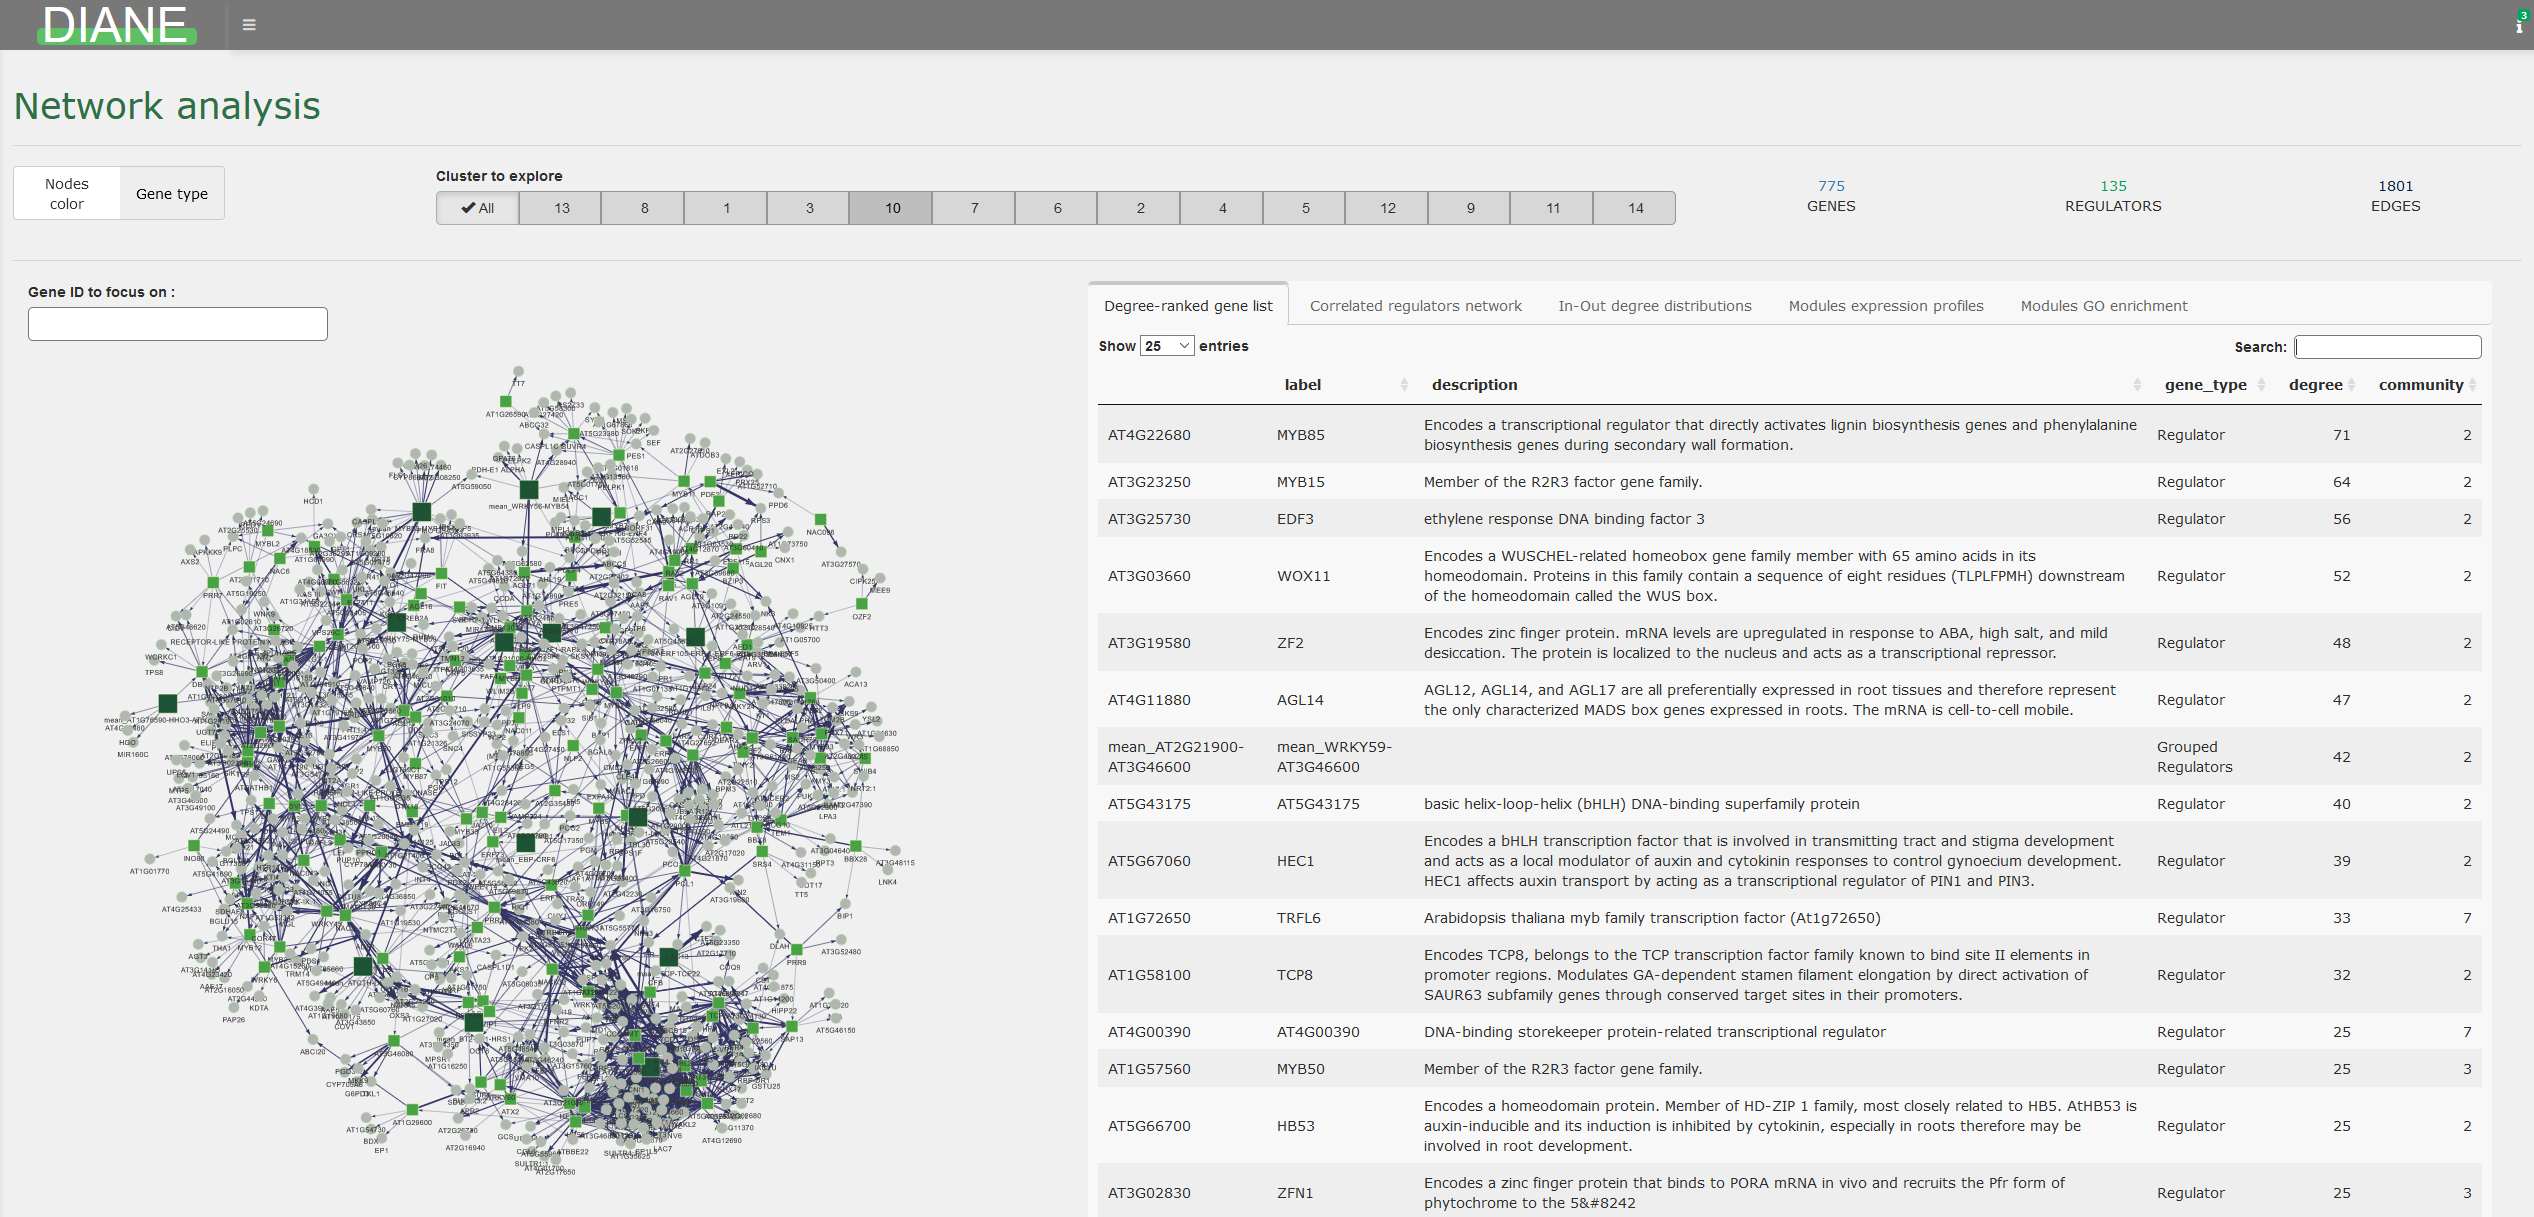
\includegraphics[scale = 0.2]{Figures/Regression/view_net.PNG}

\end{frame}






\begin{frame}{Enrichir et valider un réseau inféré}


\small Les arêtes inférées peuvent être comparées à des \textbf{liens de régulation déjà documentés}, comme :


\begin{itemize} \small 
    \item Les interactions présentes dans la \textbf{litérature}
    \item Des \textbf{données de fixation} des TFs  \textit{in vivo} ou \textit{in vitro} CHIPSeq, DAPSeq
    \item L'\textbf{accessibilité de la chromatine} et footprinting : ATACSeq
    \item La \textbf{régulation \textit{in planta}} (induction de TF dans des protoplastes \cite{Bargmann2013}, expression de gènes cibles dans des lignées de mutants, etc) 
\end{itemize}
\vspace{-0.3cm}
\onslide<2->
\begin{block}{\small Quelques efforts de regroupement en bases de données:}
\begin{itemize}\small
    \item ConnecTF \cite{Brooks2020} (Arabidopsis, maïs)
    \item AtRegNet \cite{Palaniswamy2006} (Arabidopsis)
\end{itemize}
\end{block}
\end{frame}



\begin{frame}{Enrichir et valider un réseau inféré}

\begin{columns}
\begin{column}{.5\textwidth}
\vspace{-0.1cm}
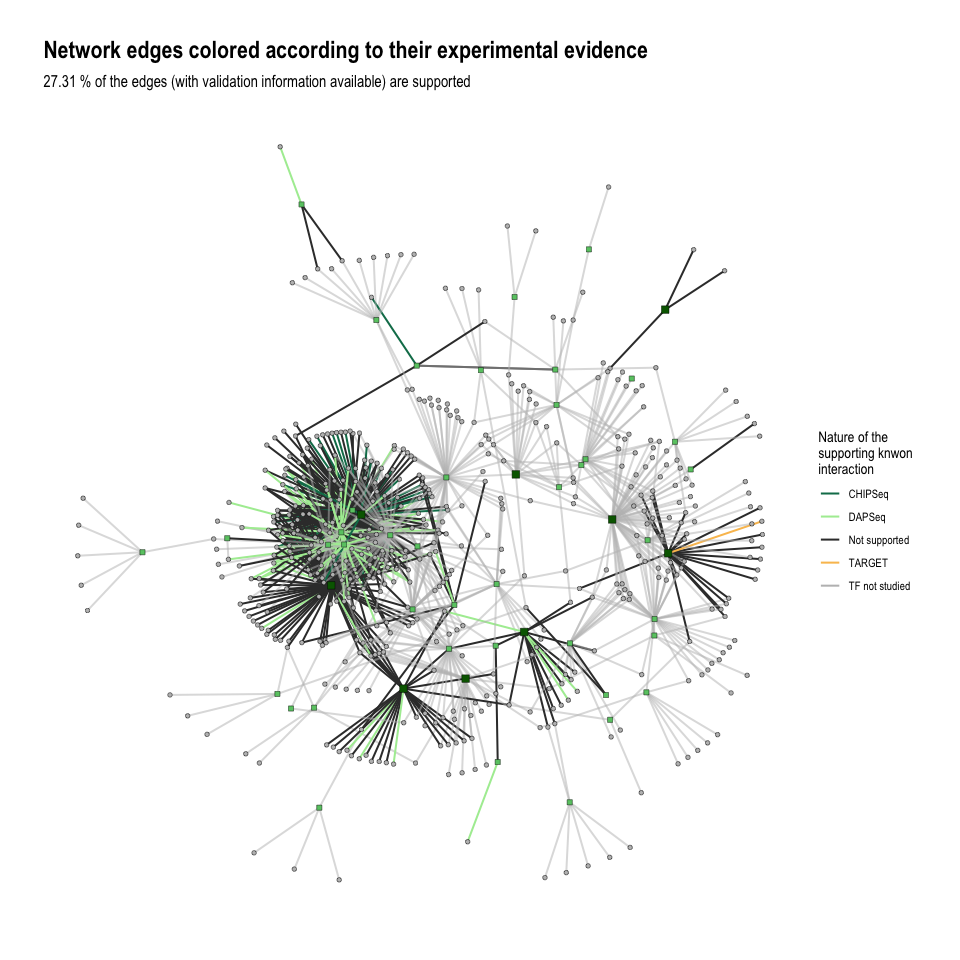
\includegraphics[scale = 0.21]{Figures/analyse/validation.png}
\end{column}
\begin{column}{.3\textwidth}
\vspace{-0.2cm}
\begin{block}{}
\scriptsize Ici, les arêtes d'un réseau prédit sont colorées suivant \textbf{leur confirmation par une expérience présente dans connecTF (DAPSeq, CHIPSeq, TARGET)}
\end{block}
\scriptsize Réseau inféré via GENIE3, validé via \href{https://oceanecsn.github.io/AraNetBench/}{AraNetBench}. \\ Arabidopsis sous stress osmotique, salin, et en température
\end{column}
\end{columns}
\end{frame}



\begin{frame}{Calculer des métriques de validation sur un réseau inféré}

\begin{columns}
\begin{column}{.48\textwidth}
\begin{itemize}\small
    \item \textbf{Vrais positifs - précision} : nombre d'arêtes prédites supportées par une information expérimentale (absolu, ou rapporté au nombre d'arêtes total qu'il est possible de valider)
    
    \item \textbf{Faux positifs, vrais négatifs, faux négatifs, rappel}
\end{itemize}
\onslide<3->
\begin{alertblock}{\small \danger Interprétation de ces métriques}\scriptsize
Ces données de validation sont \textbf{imparfaites}, elles contiennent des faux positifs, et faux négatifs : prudence
\end{alertblock}
\end{column}
\begin{column}{.48\textwidth}
\onslide<2->
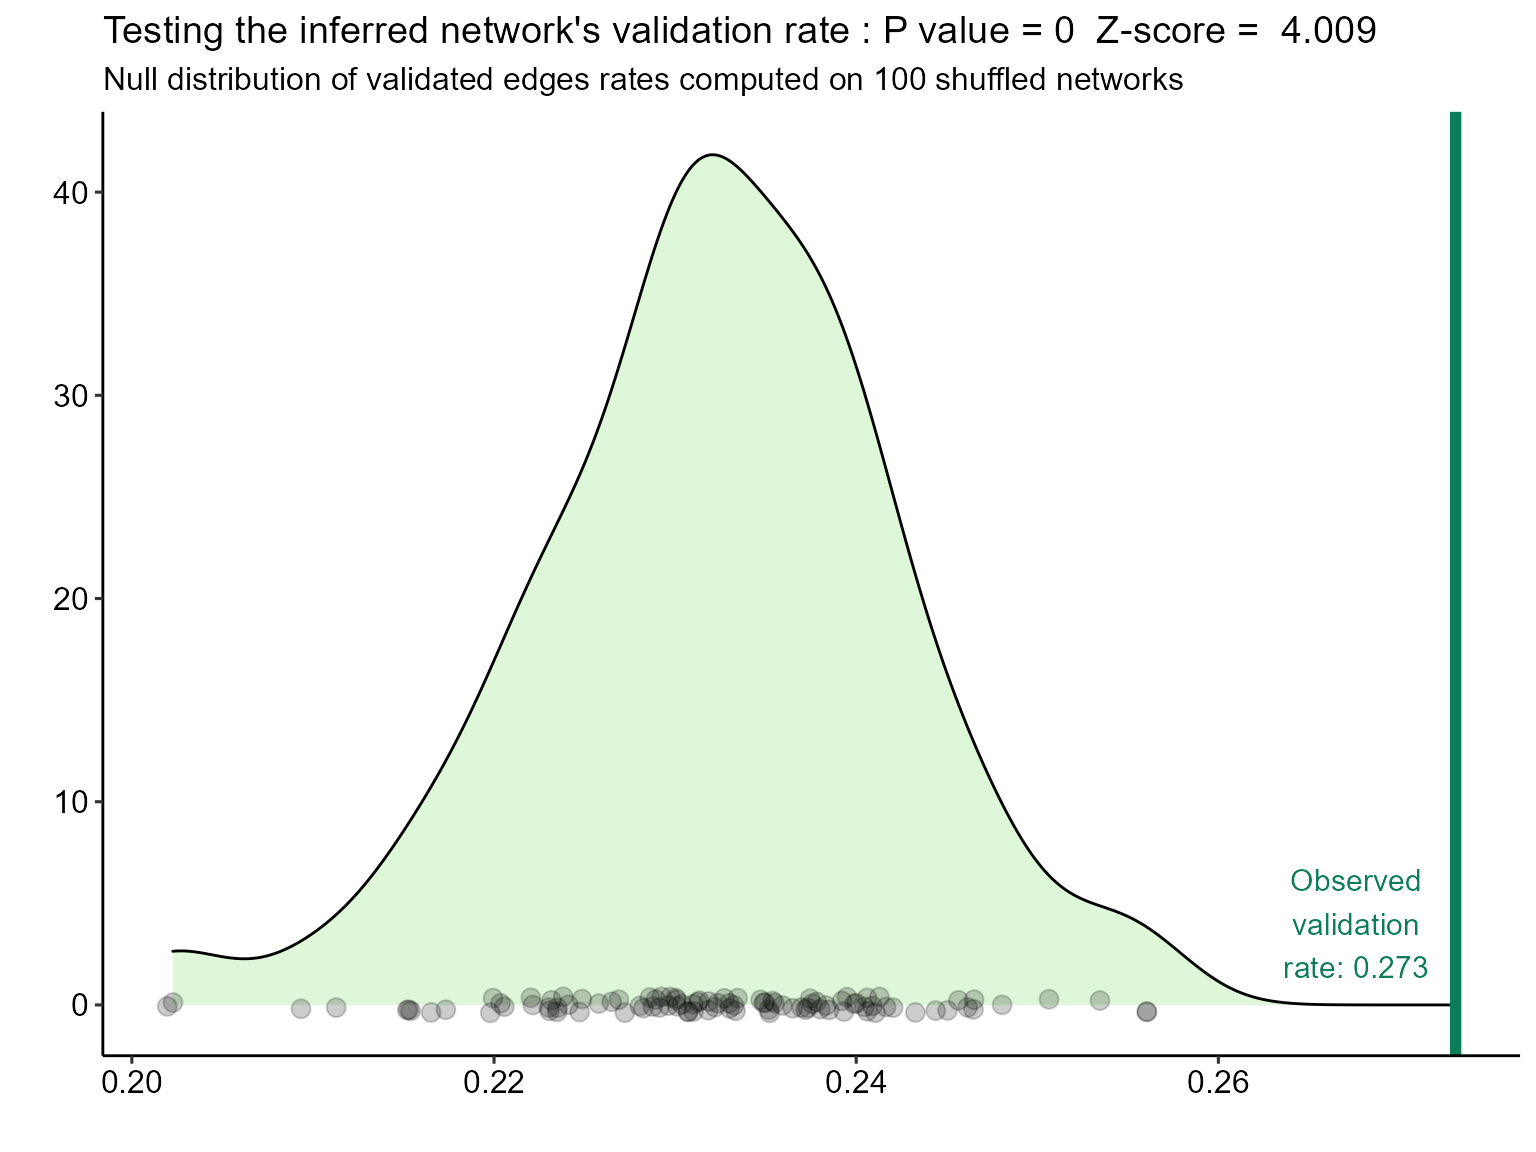
\includegraphics[scale = 0.3]{Figures/Regression/validationtest.png}
\end{column}
\end{columns}
\end{frame}



%\subsection{Analyse et validation de réseaux}



\begin{frame}{Analyser la topologie d'un réseau : détection de modules}

\begin{itemize}
    \item \small \textbf{Communautés} de gènes densément connectés, contenant des éventuels enrichissements ontologiques. \tiny{Conrad et al, BMC Syst. Biology 2018}
    \center
     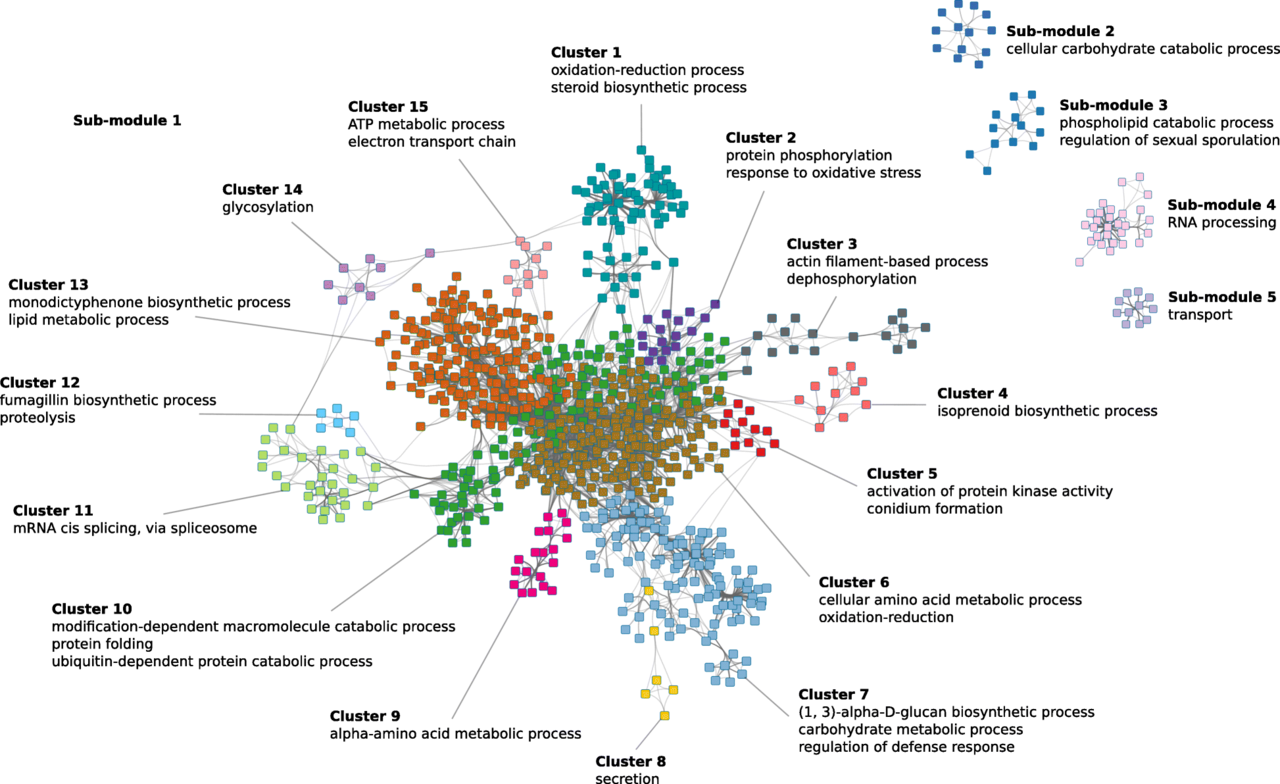
\includegraphics[scale = 0.195]{Figures/analyse/modules.png} 
     
    
\end{itemize}
	
\end{frame}


\begin{frame}{Analyser la topologie d'un réseau inféré : connectivité}

\begin{itemize}
 \item \small \textbf{Degré - centralité} : Les gènes montrant une connectivité remarquable dans le réseau sont de potentiels régulateurs clés
 
 \center
     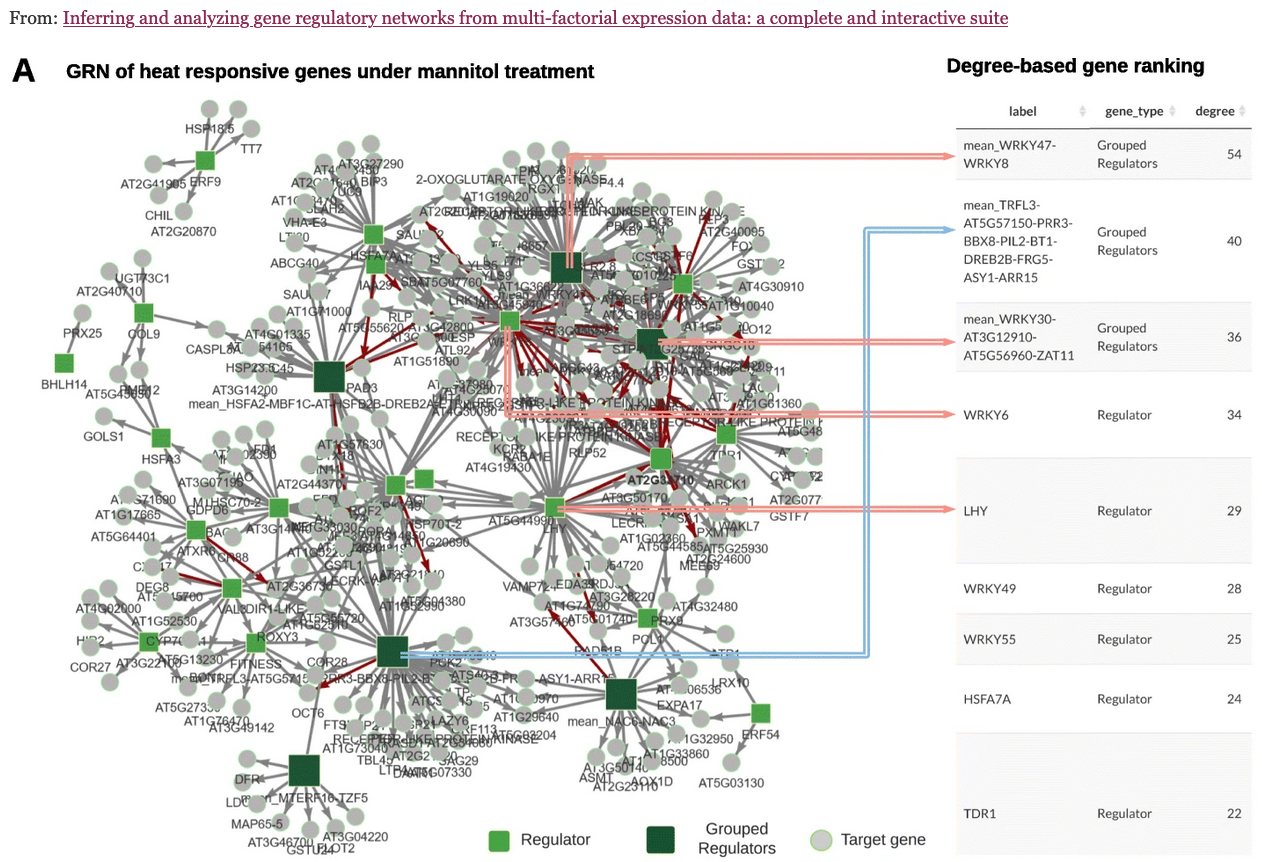
\includegraphics[scale = 0.17]{Figures/analyse/rankingTF.png}
    
\end{itemize}

\end{frame}


% conclusion / synthèse


\begin{frame}{Inférer des réseaux de régulation : un tâche encore complexe}
	
	\begin{enumerate}
	    \item Problème en grande dimension
	    
	    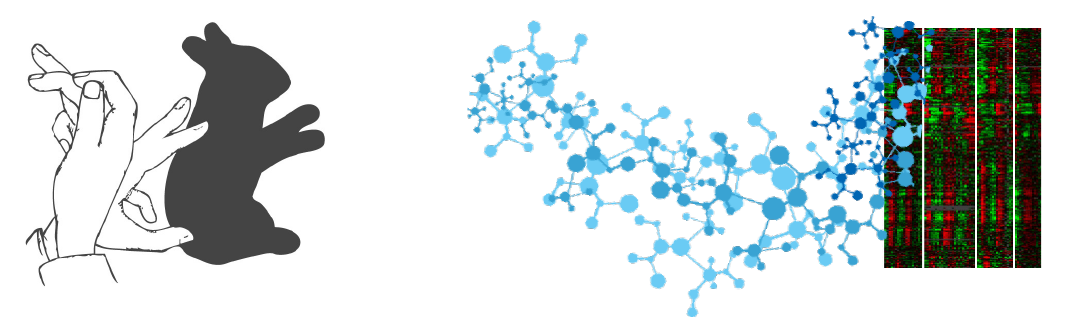
\includegraphics[scale=0.2]{Figures/Intro/shadowplay.png}
	    
	    
	    \item Manque de données de validation complètes et sûres pour étalonner les méthodes
	\end{enumerate}

\end{frame}




\begin{frame}{Combiner plusieurs approches d'inférence}

\scriptsize En 2012, les challenges \textbf{DREAM} ont évalué et combiné l'état de l'art des méthodes d'inférence  et conclu à un apport significatif de la combinaison de plusieurs méthodes [Marbach et al., 2012]

\centering
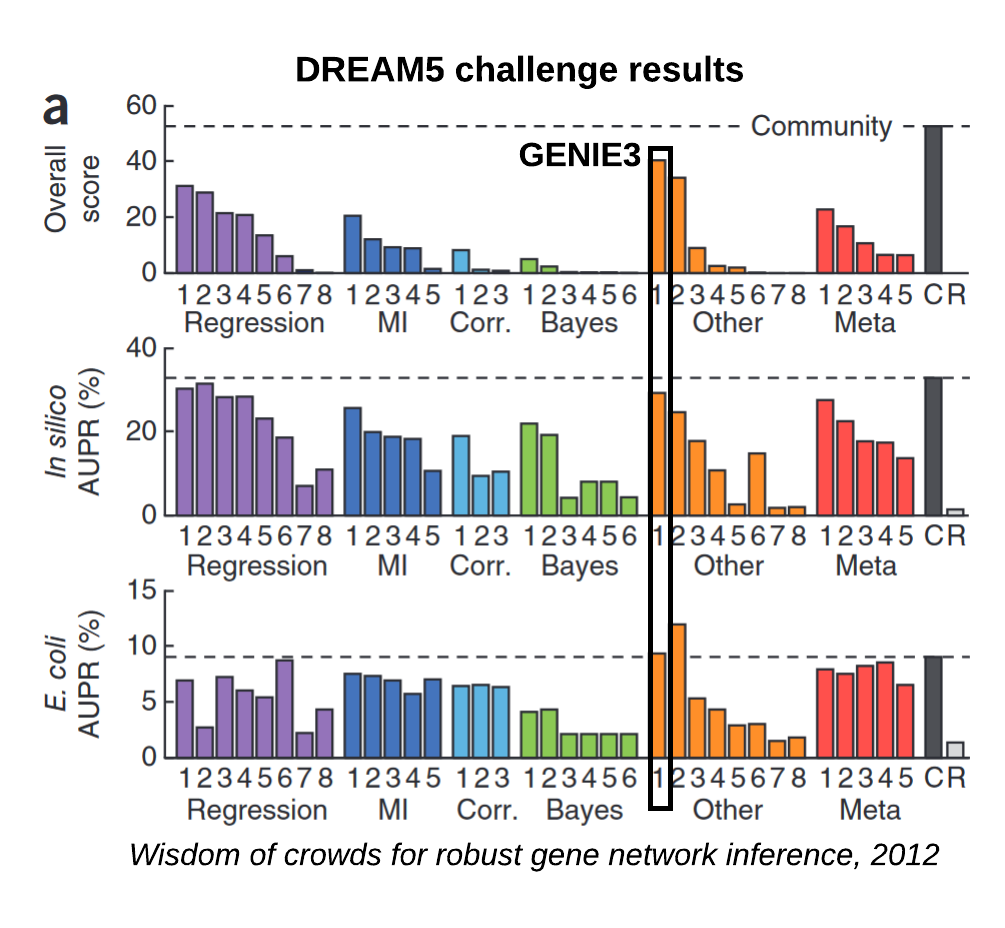
\includegraphics[scale = 0.38]{Figures/Regression/dream5.png}
\end{frame}



\begin{frame}{Utilité de ces analyses pour la biologie des systèmes}

\textbf{L'analyse des réseaux inférés peut permettre de:}
    \begin{itemize} \small
    \item Conforter et approfondir des connaissances existantes en biologie des systèmes
        \item Découvrir de nouveaux gènes candidats contrôlant des réponses d'intérêt, après validation expérimentale et étude fonctionnelle
    \end{itemize}
    
    \vspace{0.5cm}
    \begin{alertblock}{Accomplissements de l'inférence de réseaux}
	Meilleure compréhension des systèmes vivants, solutions pour améliorer la résilience d'un organisme à une contrainte environnementale ou à des pathologies
	\end{alertblock}
	
    
\end{frame}
	

